\section{Dashboard interactivo y presentación analítica}

\subsection{Arquitectura del sistema web y desacoplamiento}
La interfaz analítica fue construida mediante el microframework Flask, complementada con plantillas modulares Jinja2 y estilos en CSS puro con arquitectura de variables y tokens de color personalizados (modo oscuro y claro). El sistema implementa un desacoplamiento estricto respecto al pipeline de datos: la aplicación no interactúa directamente con el archivo crudo ni ejecuta transformaciones sobre la marcha. En su lugar, el servicio central (\texttt{dataset\_service.py}) resuelve la versión publicada leyendo el archivo de registro JSON (\texttt{registry.json}), validando la huella SHA-256 del archivo Parquet o CSV antes de suministrar datos a las vistas.

\subsection{Módulos funcionales del sistema}
La suite interactiva se compone de tres módulos centrales (ilustrados en la figura \ref{fig:dashboard_suite}):

\begin{enumerate}[leftmargin=0.5in]
  \item \textbf{Resumen ejecutivo y control de calidad (\texttt{/dashboard/calidad}):} Expone métricas antes/después, tablas de frecuencia de ausencias por variable, trazabilidad de reglas de limpieza y confirmación de que la clave relacional \texttt{(folio, nro)} presenta cero colisiones.
  \item \textbf{Explorador de universos y diccionario (\texttt{/dashboard/universo}):} Permite navegar por las 11 vistas temáticas, consultando las etiquetas oficiales del INE F27, tasas de completitud por columna y criterios de exclusión de poblaciones no elegibles.
  \item \textbf{Distribución regional y mapa interactivo (\texttt{/dashboard/region}):} Cartografía digital oficial del Estado Plurinacional de Bolivia basada en polígonos vectoriales SVG de alta precisión para los nueve departamentos.
\end{enumerate}

\begin{figure}[htbp]
\centering
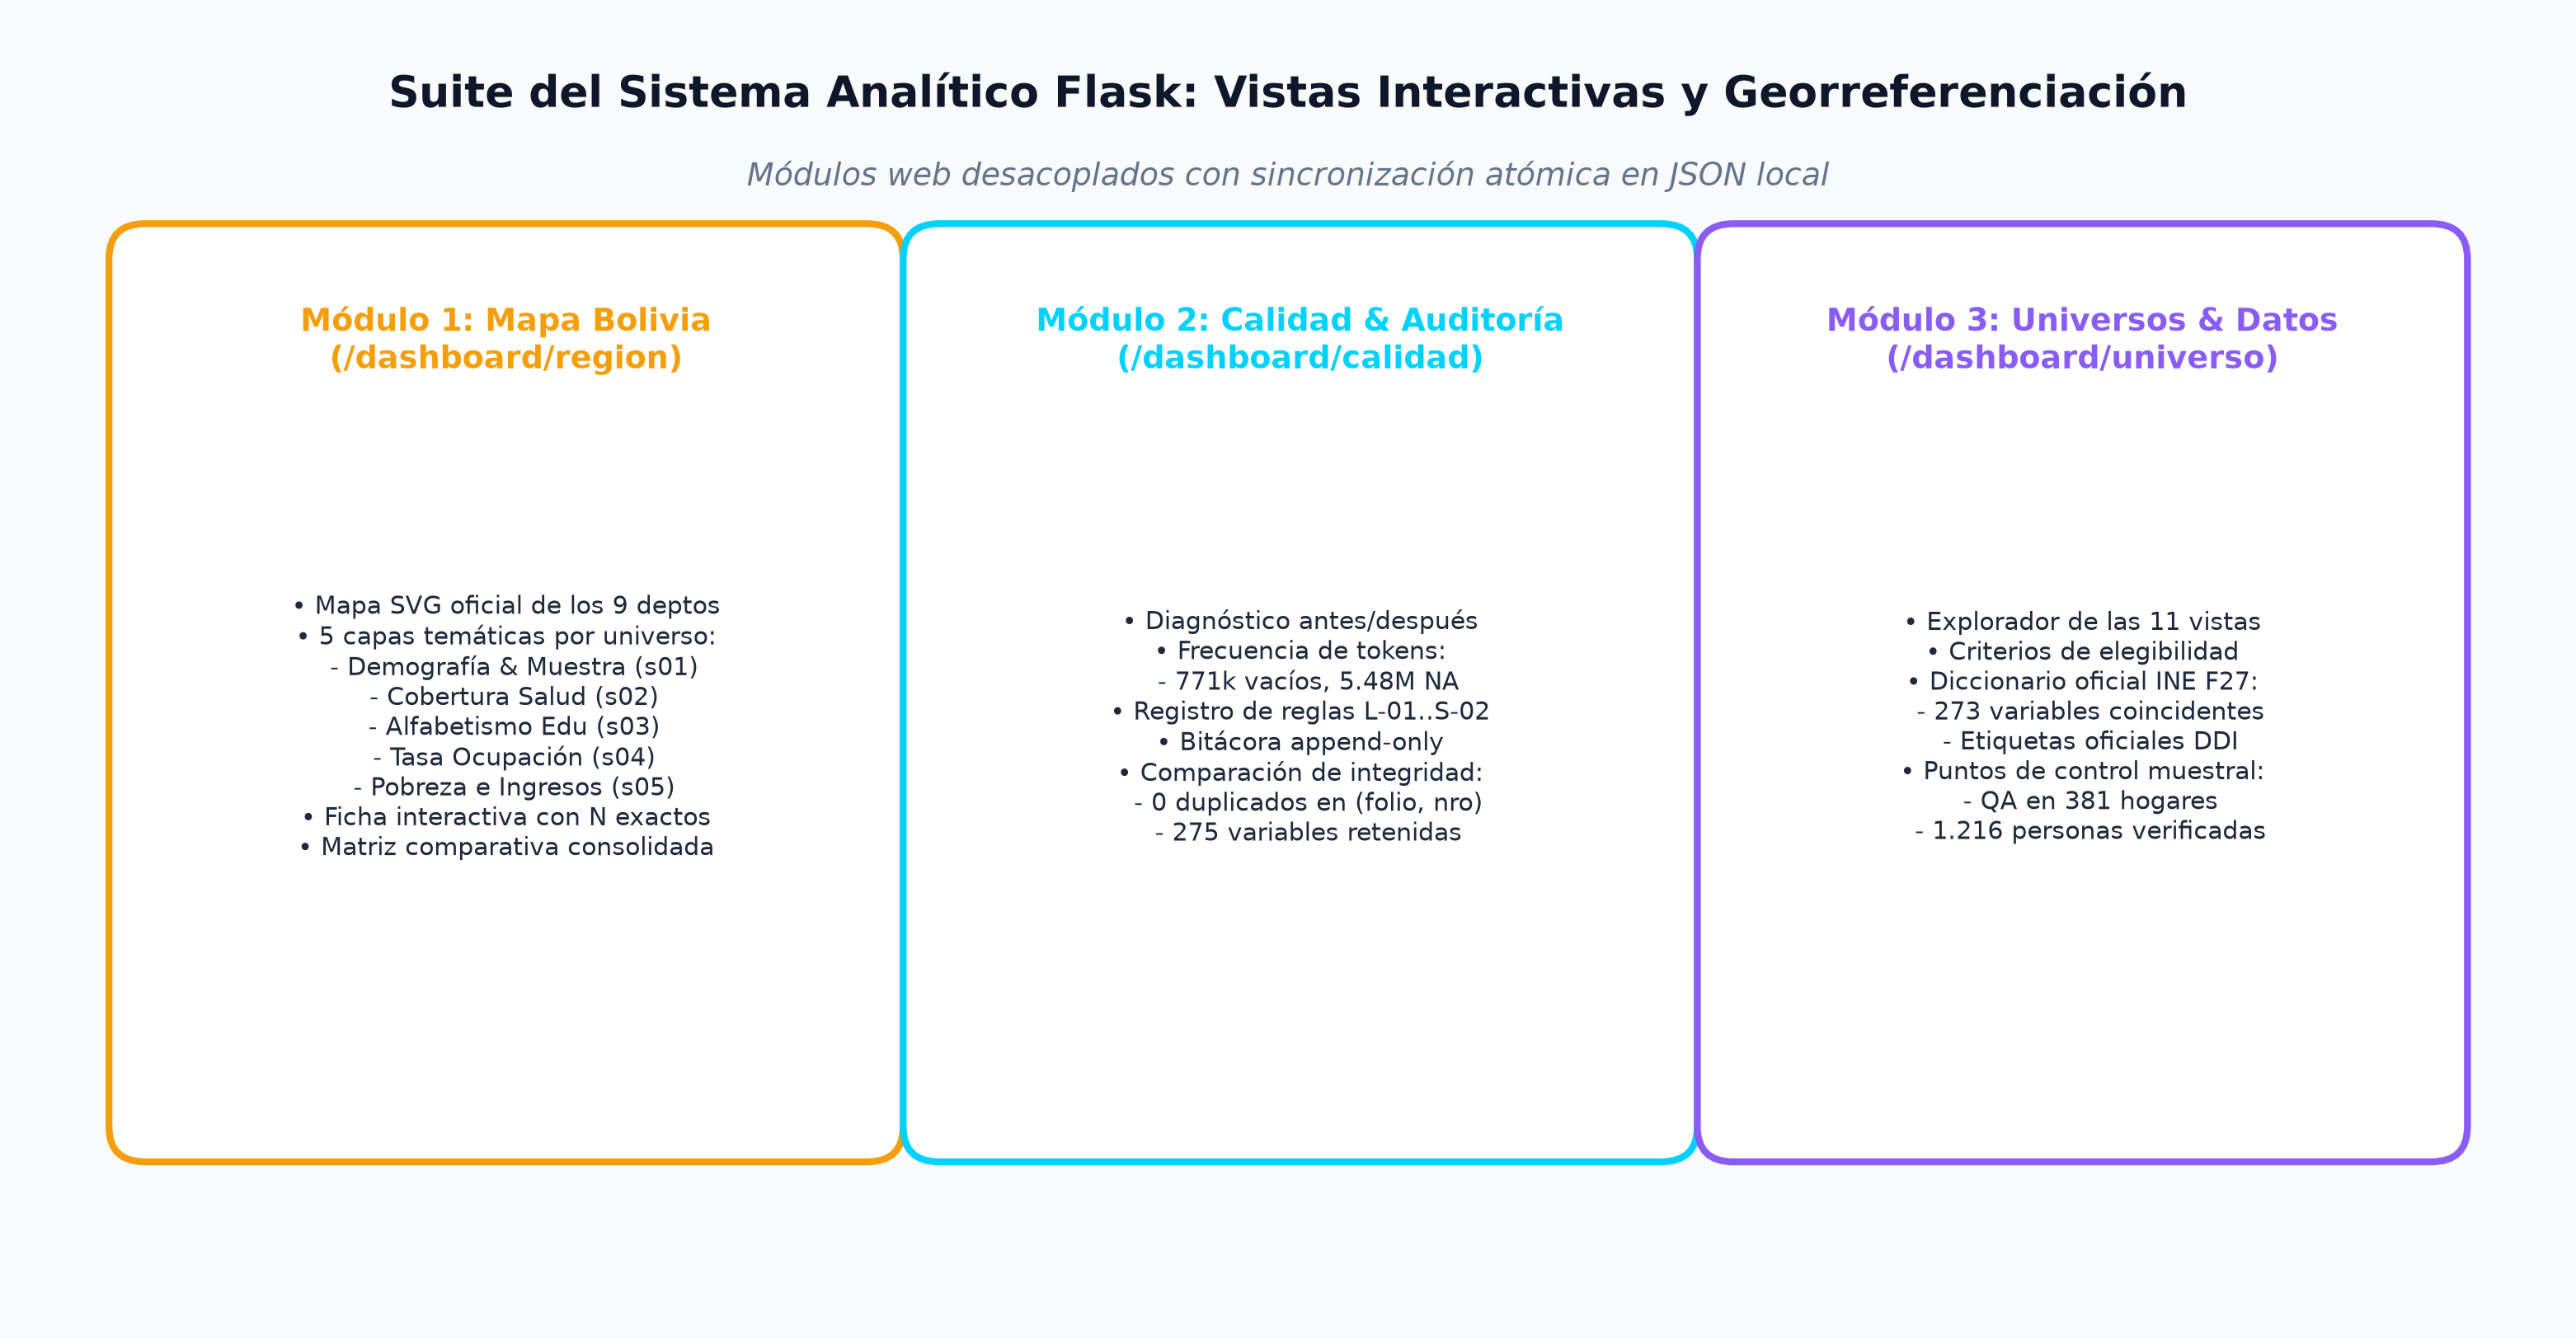
\includegraphics[width=0.98\textwidth]{figuras/fig7_dashboard_suite_capturas.png}
\caption{Suite interactiva del sistema analítico Flask: Módulos de Georreferenciación, Calidad y Universos}
\label{fig:dashboard_suite}
\par\vspace{3pt}\parbox{0.98\textwidth}{\footnotesize\textit{Nota.} Estructura modular del front-end analítico: módulo regional con mapa SVG de Bolivia, módulo de auditoría de calidad y explorador de las 11 vistas temáticas.}
\end{figure}

\subsection{Cartografía interactiva y consolidación departamental}
A diferencia de implementaciones preliminares que empleaban métricas demostrativas, el módulo regional fue completamente actualizado para consumir las cantidades estadísticas exactas calculadas directamente desde el maestro \texttt{persona\_clean\_master.parquet}. 

El mapa interactivo permite activar cinco capas temáticas dinámicas:
\begin{itemize}[leftmargin=0.5in]
  \item \textit{División Departamental Oficial (Capa Política):} Mapeo cromático de los 9 departamentos.
  \item \textit{Demografía \& Muestra ($s01$):} Densidad observada de personas y hogares encuestados.
  \item \textit{Universo Salud ($s02$):} Tasa de cobertura de seguro médico (SUS, Cajas de Salud y privados).
  \item \textit{Universo Educación ($s03$):} Tasa de alfabetismo en personas de 15 años o más.
  \item \textit{Universo Empleo ($s04$):} Tasa de ocupación en la Población en Edad de Trabajar (PET $\ge 7$ años).
  \item \textit{Universo Ingresos ($s05$):} Incidencia de pobreza moderada observada.
\end{itemize}

Al interactuar con cualquier departamento en el mapa SVG o en la tabla, el panel lateral actualiza dinámicamente las cifras de muestra observada, desglose urbano/rural, población femenina en edad fértil (MEF 13--50 años), niñez asistida y mediana del ingreso laboral líquido. La síntesis de estas métricas se presenta en la tabla \ref{tab:matriz_departamental}.

\begin{table}[htbp]
\centering
\caption{Matriz consolidada de la muestra por departamento y universos de la encuesta}
\label{tab:matriz_departamental}
\begin{tabularx}{\textwidth}{>{\raggedright\arraybackslash\small}p{2.1cm}>{\raggedleft\arraybackslash\small}p{1.35cm}>{\raggedleft\arraybackslash\small}p{1.35cm}>{\raggedleft\arraybackslash\small}p{1.75cm}>{\raggedleft\arraybackslash\small}p{1.85cm}>{\raggedleft\arraybackslash\small}p{1.65cm}>{\raggedleft\arraybackslash\small}X}
\toprule
\textbf{Depto} & \textbf{Muestra ($N$)} & \textbf{Hogares} & \textbf{Con Seguro ($s02$)} & \textbf{Alfabetos $\ge$15a ($s03$)} & \textbf{Ocupados PET ($s04$)} & \textbf{Pobres ($s05$)} \\
\midrule
Chuquisaca & 3.546 & 1.130 & 2.681 (75,6\%) & 2.351 (89,6\%) & 2.075 (64,6\%) & 1.738 (49,0\%) \\
La Paz & 9.839 & 3.251 & 6.484 (65,9\%) & 7.350 (97,9\%) & 5.411 (60,5\%) & 4.300 (43,7\%) \\
Cochabamba & 6.714 & 2.166 & 4.915 (73,2\%) & 4.972 (96,6\%) & 3.612 (59,3\%) & 2.253 (33,6\%) \\
Oruro & 2.803 & 952 & 2.189 (78,1\%) & 2.048 (97,1\%) & 1.610 (63,8\%) & 995 (35,5\%) \\
Potosí & 3.522 & 1.133 & 2.877 (81,7\%) & 2.311 (91,1\%) & 1.894 (61,0\%) & 1.972 (56,0\%) \\
Tarija & 2.514 & 832 & 2.277 (90,6\%) & 1.817 (95,7\%) & 1.378 (60,6\%) & 802 (31,9\%) \\
Santa Cruz & 6.991 & 2.028 & 4.153 (59,4\%) & 5.021 (98,0\%) & 3.788 (60,8\%) & 1.587 (22,7\%) \\
Beni & 2.591 & 718 & 2.044 (78,9\%) & 1.789 (97,8\%) & 1.332 (58,3\%) & 933 (36,0\%) \\
Pando & 1.977 & 508 & 1.479 (74,8\%) & 1.305 (98,3\%) & 1.209 (71,0\%) & 731 (37,0\%) \\
\midrule
\textbf{Total} & \textbf{39.497} & \textbf{12.718} & \textbf{29.099 (73,7\%)} & \textbf{28.964 (96,3\%)} & \textbf{22.309 (61,3\%)} & \textbf{15.311 (38,8\%)} \\
\bottomrule
\end{tabularx}
\par\vspace{3pt}\parbox{\textwidth}{\footnotesize\textit{Nota.} Conteos exactos de la muestra observada. Las tasas departamentales corresponden a la población elegible evaluada en cada módulo de la encuesta. Fuente: \texttt{departamentos\_full\_stats.json}.}
\end{table}

\subsection{Políticas de privacidad y supresión de celdas pequeñas}
Para evitar la reidentificación de personas o informantes en celdas estadísticas desagregadas, el servicio de visualización aplica una regla estricta de supresión de umbral: cualquier categoría con menos de 10 registros individuales observados se suprime de los gráficos públicos. Adicionalmente, se ejecuta supresión complementaria en la categoría de menor frecuencia contigua para impedir que el usuario deduzca el valor oculto a partir del total marginal $N$.
